\chapter{Worked examples}

Four programs that do real work. Each was run against the tree while this
chapter was written; the transcripts are the actual output.

\section{Log triage: regular expressions, done Poplog's way}

Poplog ships a full regexp engine (\code{ref regexp}) --- but with inverted
syntax, and this catches everyone exactly once. \textbf{The escape character
is \code{@}, not backslash, and \code{.\ * [ ] \^{} \$} are literal by
default.} A pattern pasted in from any other engine compiles without
complaint and then matches almost nothing.

\begin{center}
\footnotesize
\begin{tabular}{llll}
\toprule
\textbf{PCRE} & \textbf{Poplog} & \textbf{PCRE} & \textbf{Poplog}\\
\midrule
\code{.} & \code{@.} & \code{x?} & \code{x@\{0,1@\}}\\
\code{*} & \code{@*} & \code{x\{m,n\}} & \code{x@\{m,n@\}}\\
\code{[abc]} & \code{@[abc@]} & \code{\^{}} \ \code{\$} & \code{@\^{}} \ \code{@\$}\\
\code{x+} & \code{x@\{1,@\}} & \code{(x)} & \code{@(x@)}\\
\bottomrule
\end{tabular}
\end{center}

There is no alternation (\code{|}) and no lookaround: compile one pattern per
branch. In exchange, \code{regexp\_compile} hands back a \emph{compiled
procedure} you define once and then call at native speed.

\begin{pop}
;;; triage.p -- count log levels and find the slowest reported query
uses regexp;

vars err, match_ms;
regexp_compile('@[0-9@]@{1,@} ms') -> (err, match_ms);
if err then mishap(err, 0, 'bad pattern') endif;

define triage(path) -> (counts, slowest);
    lvars dev, rep, line, lev, i, n, ms;
    newproperty([], 8, 0, true) -> counts;     ;;; default 0, so += just works
    0 -> slowest;
    sysopen(path, 0, "line") -> dev;
    line_repeater(dev, inits(4096)) -> rep;    ;;; size the buffer generously
    repeat
        rep() -> line;
        quitif(line == termin);
        for lev in [INFO WARN ERROR] do
            if issubstring(lev sys_>< '', 1, line) then
                counts(lev) + 1 -> counts(lev)
            endif
        endfor;
        match_ms(1, line, false, false) -> (i, n);
        if i then
            strnumber(substring(i, n - 3, line)) -> ms;
            if ms and ms > slowest then ms -> slowest endif
        endif;
    endrepeat;
enddefine;
\end{pop}

Against a seven-line sample log:

\begin{repl}
INFO: 2
WARN: 2
ERROR: 3
slowest query: 1420 ms
\end{repl}

Two idioms are doing quiet work here. \code{newproperty([], 8, 0, true)}
gives a table whose \emph{default is 0}, so incrementing an unseen key needs
no initialisation branch. And \code{line\_repeater} returns a procedure that
yields one line per call and \code{termin} at end of file --- the standard
Poplog shape for a stream, and the same shape \code{sys\_obey\_linerep} uses
for the output of a shell command.

\section{A web service in pure Pop-11}

\code{lib http\_server} and \code{lib json} compose into a service with
routing, query and body access, and the usual safety nets --- an unknown
route answers 404, and a mishap inside a handler answers 500 without taking
the server down. The whole program is the handler.

\begin{pop}
uses http_server;
uses json;

define handler(req) -> resp;
    lvars path = req('path'), obj;
    if path = '/hello' then
        http_text('hello from Pop-11\n') -> resp;
    elseif path = '/greet' then
        newmapping([], 4, false, true) -> obj;
        req('query')  -> obj('query');
        req('method') -> obj('method');
        http_json(obj) -> resp;
    elseif path = '/info' then
        newmapping([], 4, false, true) -> obj;
        'poplog' -> obj('server');
        pop_internal_version -> obj('version');
        http_json(obj) -> resp;
    elseif path = '/boom' then
        mishap(0, 'deliberate handler failure');   ;;; server answers 500
    else
        false -> resp;                             ;;; server answers 404
    endif;
enddefine;

http_serve_n(8099, handler, false);
\end{pop}

\begin{repl}
$ curl -s localhost:8099/hello
hello from Pop-11
$ curl -s 'localhost:8099/greet?name=poplog'
{"method":"GET","query":"name=poplog"}
$ curl -s localhost:8099/info
{"version":160200,"server":"poplog"}
$ curl -s -o /dev/null -w '%{http_code}\n' localhost:8099/nope
404
\end{repl}

\code{lib json} maps JSON onto Pop-11 directly: an object becomes a
\code{newmapping} property, an array a vector, a string a string of UTF-8
bytes, and \code{null} the distinguished word \code{json\_null} (kept apart
from \code{false}, which is JSON \code{false}).

\begin{pop}
uses json;
vars v = json_parse('{"name": "poplog", "ports": [64, 32]}');
v('name')      =>        ;;; ** poplog
v('ports')(1)  =>        ;;; ** 64
json_generate(v) =>      ;;; ** {"ports":[64,32],"name":"poplog"}
\end{pop}

Object member order is not preserved --- properties are hash tables, and
RFC~8259 promises nothing about ordering. The file is
\code{examples/http\_hello.p}; \code{teach json} walks through how
\code{lib json} itself was built, bug included.

\section{ELIZA, with the real machinery}

\code{examples/eliza.p} implements Weizenbaum's 1966 DOCTOR properly ---
keyword ranking, decomposition rules with wildcards and synonym classes,
reassembly templates cycled round-robin, pronoun reflection, \code{goto}
equivalence, and the \textsc{memory} mechanism that stows what you said about
``my \ldots'' and brings it back later. The script lives in a separate data
file, \code{doctor.txt}, exactly as Weizenbaum separated script from engine.

The reason it fits in a couple of dozen lines of matching logic is
\S3.8's matcher: a decomposition rule \emph{is} a Pop-11 list pattern.

\begin{repl}
How do you do.  Please tell me your problem.
    Well, my boyfriend made me come here.
Your boyfriend made you come here?
    He says I am depressed much of the time.
I am sorry to hear that you are depressed.
    My mother takes care of me.
Tell me more about your family.
    It is raining today.            <- no keyword: a stored memory returns
Lets discuss further why your mother takes care of you.
\end{repl}


\section{Graphics, briefly}

Poplog's graphics were historically tied to X. This fork adds an optional
native backend built on Dear ImGui, chosen at build time with
\code{./configure --experimental-graphics}: Metal + Cocoa on macOS, or SDL3 +
OpenGL3 on macOS or Linux --- and SDL3 picks its display transport at run
time, so Wayland, X11, KMS/DRM and headless software rendering all work from
one build. The classic \code{rc\_graphic} turtle library and \code{rc\_mouse}
are ported onto it, so existing Pop-11 graphics code runs unchanged.

\begin{figure}[h]
\centering
\begin{minipage}[t]{0.47\linewidth}\centering
  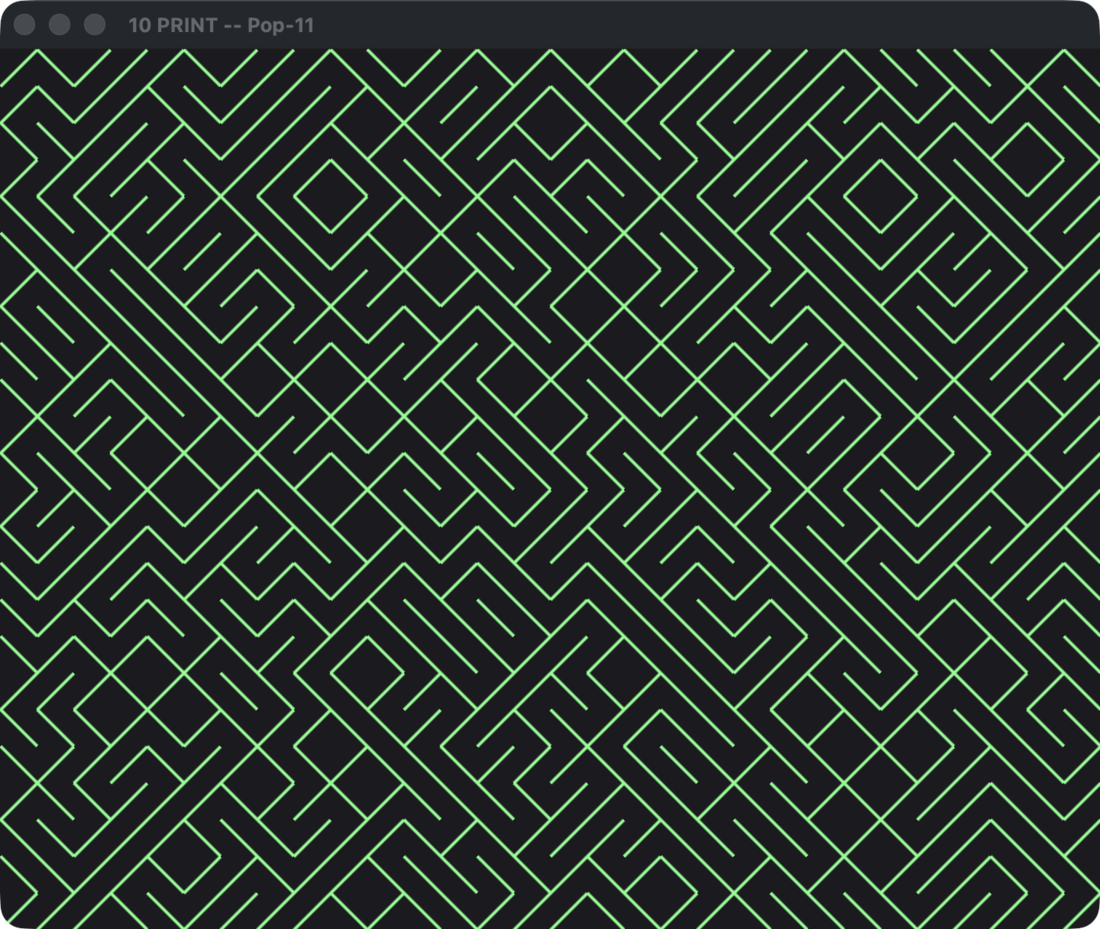
\includegraphics[width=\linewidth]{figures/ex-tenprint}\\[3pt]
  {\footnotesize\sffamily\color{popgrey}\code{examples/tenprint.p} --- the 10 PRINT maze}
\end{minipage}\hfill
\begin{minipage}[t]{0.47\linewidth}\centering
  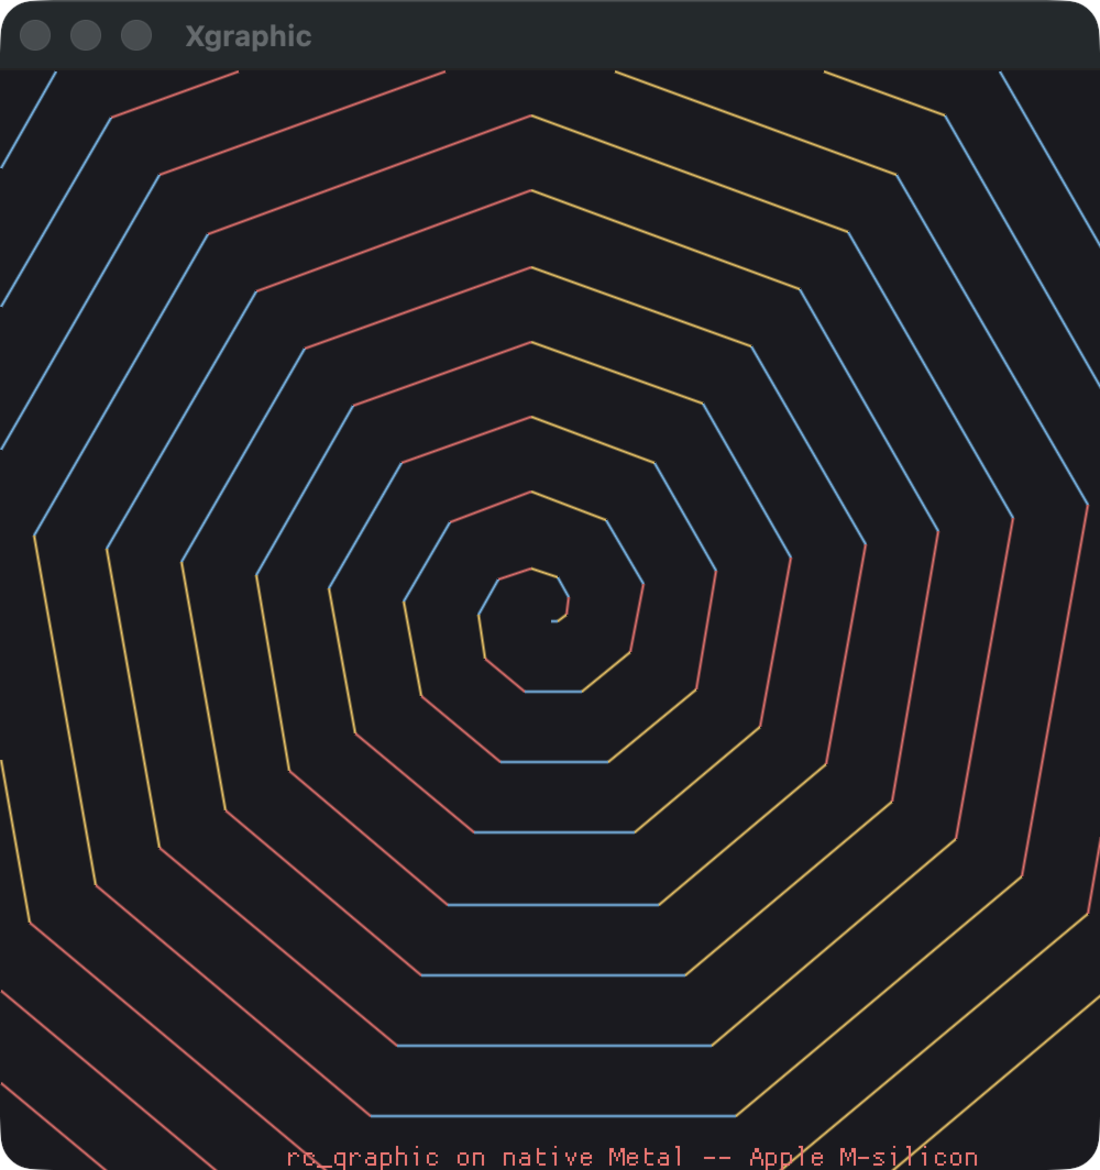
\includegraphics[width=\linewidth]{figures/graphics-macos}\\[3pt]
  {\footnotesize\sffamily\color{popgrey}\code{rc\_graphic} turtle on the Metal backend}
\end{minipage}
\end{figure}

Graphics are strictly opt-in: the default build, and \code{nix build
.\#poplog}, are console-only.

\section{Working against a live image}

The last example is not a program but a habit. Because compiling is
microseconds and saving the heap is milliseconds, the natural unit of work is
a \emph{session} that accumulates state, with snapshots at the points worth
returning to.

\begin{repl}
$ popsession start --name triage            # boot a session (~50 ms)
$ popsession send  --name triage -f triage.p       # define the helpers once
$ popsession send  --name triage -c "triage('app.log') =>"     # ~1 ms per call
$ popsession checkpoint --name triage scan-v1.psv  # freeze heap + procedures
$ popsession restore    --name triage scan-v1.psv  # a new process, fully loaded
\end{repl}

The image contains the compiled procedures, so restoring is not re-loading:

\begin{repl}
$ ls -lh session.psv
2.9M session.psv              # a heap holding 10,000 compiled procedures
$ time popsession restore session.psv
0.064 total                   # including process spawn
$ gen_9999(1) =>
** 10000
\end{repl}

Two cautions, both from \S1.4. A restore rolls the \emph{whole} session back
--- anything defined after the snapshot is gone, so re-checkpoint after adding
to a restored session. And handles into the operating system or into C
libraries go stale across a restore; reopen them rather than trusting them.
